\subsection{Peculiar velocity 2}
Upcoming wide field surveys will find a large number of supernovae, and will have the ability to trace large scale structure. The best methods to do so need to be explored. In particular, the interesting methods will probably use both the distance  scales measured by supernovae using their standard candle properties and their properties as tracers of large scale structure simultaneously for the same supernova. One such probe is a probe of peculiar velocity correlations using SNIa, where the standard candle property is used to derive the distance scale, while the measured redshift (spectroscopic or photometric) is used simultaneously to gauge the peculiar velocity of the SNIa (which is potentially the peculiar velocity of the host galaxy). The spatial correlation of such peculiar velocities is related to the matter over-density at the location through the Poisson Equations, and thus can be used to constrain the over-densities and the growth function. This can be used to constrain the cosmology (for example, see \cite{2011PhRvD..83d3004B}). For other computational approaches to similar science cases, such as \cite{howlett}.

\myparagraph{Method}

In what follows, we heavily rely on \cite{2011PhRvD..83d3004B}. We wish to estimate the uncertainties in the estimate of pairwise velocities as a function of the comoving separation in bins of redshift. The expected signal is largest at low redshift, where the signal of the peculiar velocity is large compared to the recession velocity of the Hubble flow.  The uncertainty on the estimated pair-wise radial velocities of tracers separated by a comoving distance $r$ Mpc is given by
\begin{equation}
v_{\rm{est}} \approx 2 \times \sigma_{v_{\rm{los}}} / N^{1/2}(r, z_{\rm{cosmo}})
\end{equation}
where $N(r,z_{cosmo})$ is the number of pairs of SNIa separated by a comoving distance of $r~\rm{Mpc}$
at a cosmological redshift of $z_{\rm{cosmo}},$ and $\sigma_{v_{\rm{los}}}$ is the uncertanty in the
measurement of the line of sight velocity of SNIa. Thus, estimating the signal-to-noise ratio depends on the size of both of these quantities $N(r, z_{cosmo})$ and $\sigma_{v_{\rm{los}}}.$ The former depends on the number of such SNIa pairs in the universe, and the survey parameters that determine the number of detected SNIa pairs. The second quantity is dependent on the uncertainty of the measured distance modulus of individual SNIa, which for low redshift supernovae of interest is largely a combination of the intrinsic dispersion known to be $\sim \mathcal{O}(0.1)$ mag, and an uncertainty due to the fitting of light curves. In what follows, we describe how we determine these quantities for different cadences. 

First, we estimate the number of pairs of detected SNIa at a given comoving separation in redshift bins. To do so, we need a realization of SNIa positions and velocities in the universe that are consistent with the underlying correlations in large scale structure. To obtain these correlations, we start from an extra-galactic catalog based on large-scale structure simulations. We add SNIa in the galaxies of the simulated extra-galactic catalog using a prescription based on some observed relationships of the SNIa - host galaxy connection. The SNIa-host galaxy connection is an area of active research from large SNIa surveys; consequently all the host galaxy properties observed are not found in the extra-galactic catalogs we can use. Consequently, we start with a simple realization prescription based on known aspects of the connection and easily observed properties of SNIa. This preserves two gross properties of SNIa distributions: the volumetric abundance rate as a function of redshift and the fact that SNIa are more abundant in galaxies with larger stellar mass. As a result of this work, we obtain a catalog of SNIa over a sky area of $A_{cat}.$ In Fig.~\ref{fig:catalog_area}, we show the region of the sky in which we have these supernovae. In Table.~\ref{tab:numpairscat}, we show the number of pairs of SNIa at separations of $r$ Mpc in the lowest redshift bin of $z < 0.1.$

\begin{figure}
    \begin{center}
        %\scalebox{1.}
        {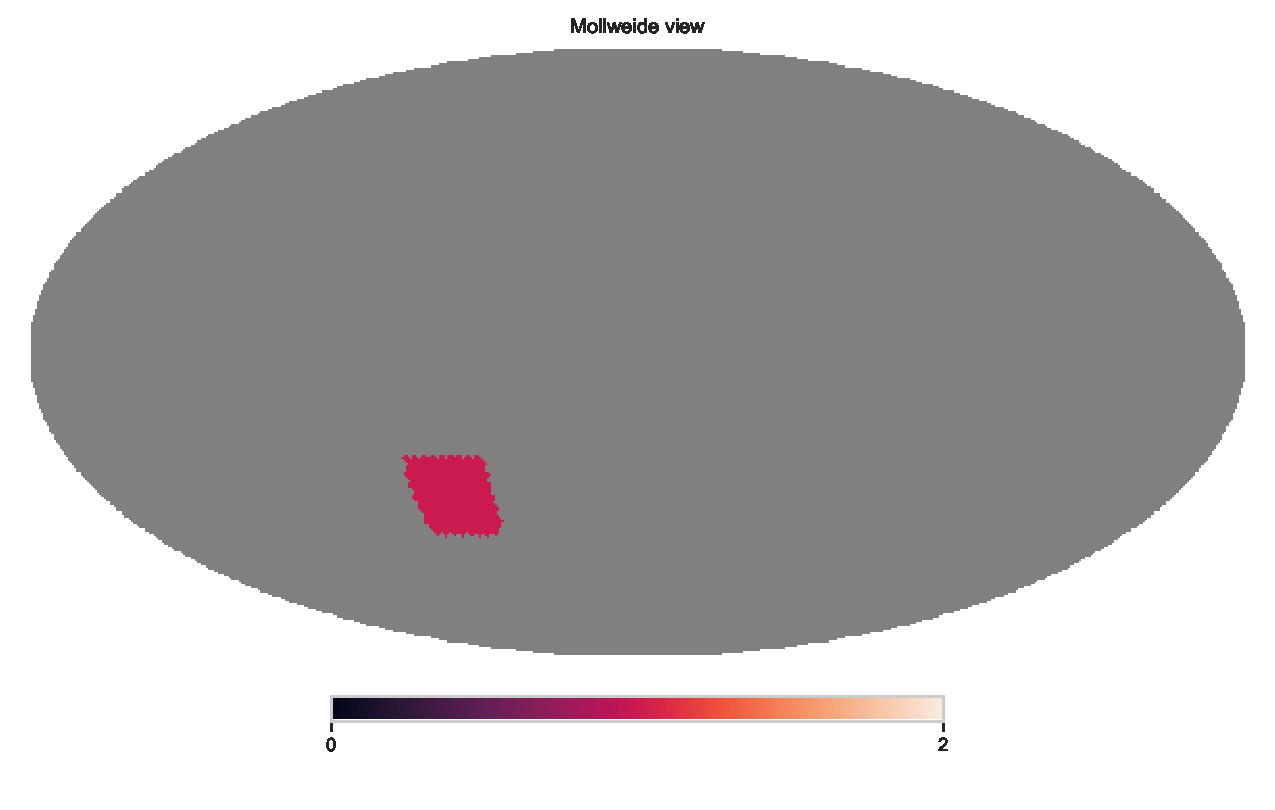
\includegraphics[width=0.4\textwidth]{peculiar_velocity/catalog_area.pdf}}
        \caption{Area of the sky covered by the extra galactic catalog used (DC2)}
        \label{fig:catalog_area}
    \end{center}
\end{figure}

\begin{table}
\begin{center}
\begin{tabular}{|c|c|}
    \hline
    $r$ (Mpc) &  Number of pairs \\
\hline
  5.0 &  1200 \\
 10.0 &  1300 \\
 15.0 &  1000 \\
 20.0 &   800 \\
 25.0 &   600 \\
 30.0 &   550 \\
 35.0 &   375 \\
 40.0 &   190 \\
 45.0 &    20 \\
 50.0 &     0 \\
\hline
\end{tabular}
\end{center}
\caption{Number of pairs found in catalog area of DC2}
\label{tab:numpairscat}
\end{table}




\begin{figure}
    \begin{center}
        %\scalebox{1.}
        {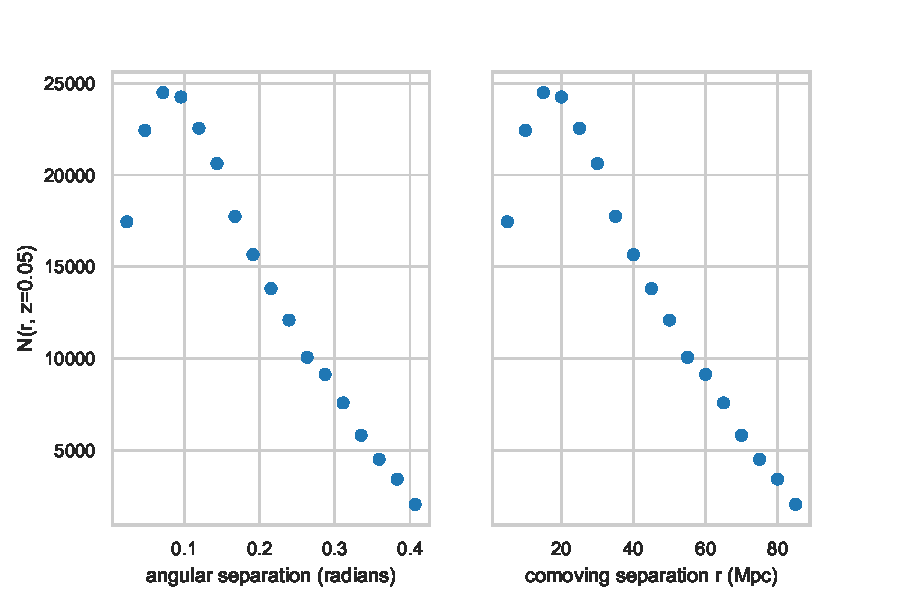
\includegraphics[width=0.4\textwidth]{peculiar_velocity/NumberPairsatDistance_z0p05.pdf}}
        \caption{Number of pairs of SNIa in the extra galactic catalog }
         \label{fig:num_pairs_cat}
    \end{center}
\end{figure}

\myparagraph{Results}

Rather than sun dedicated simulations of SNIa for this estimate, we parametrize the system by a median efficiency of detection $\epsilon = N_{det}/N_{sim}$ from other comprehensive simulations being used for supernova cadence studies, which are in turn related to a footprint area $A_{survey}$ covered by the particular observing strategy. For our purposes, we choose the footprint area to be the area of the sky where the observing strategy has at least $500$ visits over ten years, because this is the region over which the SNANA simulations run.
Therefore, we work out how the number of detected pairs scale with $A_{survey}$ and $\epsilon$ and use this information to correct the theoretical values in $N_{pairs}$ counted in the extra-galactic catalog SN. We know that the number of SNIa scales with volume in the rest frame of the SN, and thus the numbers of both detected and simulated SN are proportional to the survey area. The number of pairs of SNIa separated by a distance $r$ Mpc can be found by iterating through the SNIa ($\sim N_{SN}$), and finding the number of SNIa lying in a shell of radius $r$ Mpc with a thickness $dr$ Mpc around it, and dividing by two to avoid double counting. Using the number density of detected SN $n^{det}_{SN} \equiv N_{det}/Vol = \epsilon N_{SN}/Vol = \epsilon n_{SN},$ where $n_{SN}$ is the number density of the SNIa independent of survey parameters. We can write the number of pairs of detected SNIa with separation $r$ Mpc as 
%\begin{equation}
    $$
    N_{pairs} \propto N_{det} \times {n_{det}} \propto A_{survey} \epsilon^2 {n_{SN}}.
    $$
%\end{equation}
Thus, the estimate for number of pairs is given by
%\begin{equation}
$$
    \hat{N}_{pairs} = \left( A_{survey} / A_{catalog} \right)\hat{\epsilon}^2 \times N_{pairs}^{catalog}
    $$
%\end{equation}
where the estimate $\hat{\epsilon}$ comes from the ratio $N_{det}/ N_{simulated}$ in SNANA. 

We now consider the light curve quality with and without ground-based follow up.
If we were to get perfect light curves with lots of well observed points, as might be obtained if all low-$z$ SNIa are followed up photometrically with a different telescoper, then the appropriate metric is 
\begin{equation}
    m_{follow} \propto A_{survey} \times \epsilon^2,
\end{equation}
while if LSST is the only photometric instrument, the appropriate metric is
\begin{equation}
    m_{LSST} \propto A_{survey} \epsilon^2 /(1.0 + \left(\sigma_{lc}/0.1\right)^2)^{1/2}
\end{equation}. We calculate these metrics in Tab.~\ref{tab:cadence_metrics} and show these in Fig.~\ref{fig:cadence_metrics}



\begin{table}
\begin{center}
\begin{tabular}{|c|c|c|}
    \hline
     cadence &  Metric (photo follow-up) &  metric (LSST Only) \\
     \hline
     pontus\_2489 &         4.131681 &     2.602565 \\
     kraken\_2036 &         2.696759 &     1.637113 \\
   colossus\_2664 &         3.617946 &     2.229529 \\
     pontus\_2502 &         3.147150 &     1.910531 \\
   colossus\_2667 &         4.228459 &     2.677912 \\
     kraken\_2026 &         3.603123 &     2.231208 \\
   colossus\_2665 &         3.558642 &     2.192984 \\
     kraken\_2035 &         3.638301 &     2.242073 \\
     pontus\_2002 &         3.721372 &     2.248261 \\
     mothra\_2045 &         2.465604 &     1.495344 \\
     mothra\_2049 &         3.119186 &     1.890817 \\
     kraken\_2044 &         4.355133 &     2.700822 \\
      nexus\_2097 &         3.047014 &     1.832897 \\
     kraken\_2042 &         3.714791 &     2.305959 \\
     \hline
\end{tabular}
\end{center}
\caption{Peculiar velocity metrics for various cadences: Here `photo follow-up` implies that light curves of d
etected supernovae are perfect due to photometric follow-up with a different telescope. The right hand column 
gives the metric `(LSST Only)', where only LSST observations are assumed; the uncertainty on the distance modu
lus comes from the median uncertainty from LSST-only fits.}
\label{tab:cadence_metrics}
\end{table}

\begin{figure}
    \begin{center}
        %\scalebox{1.}
        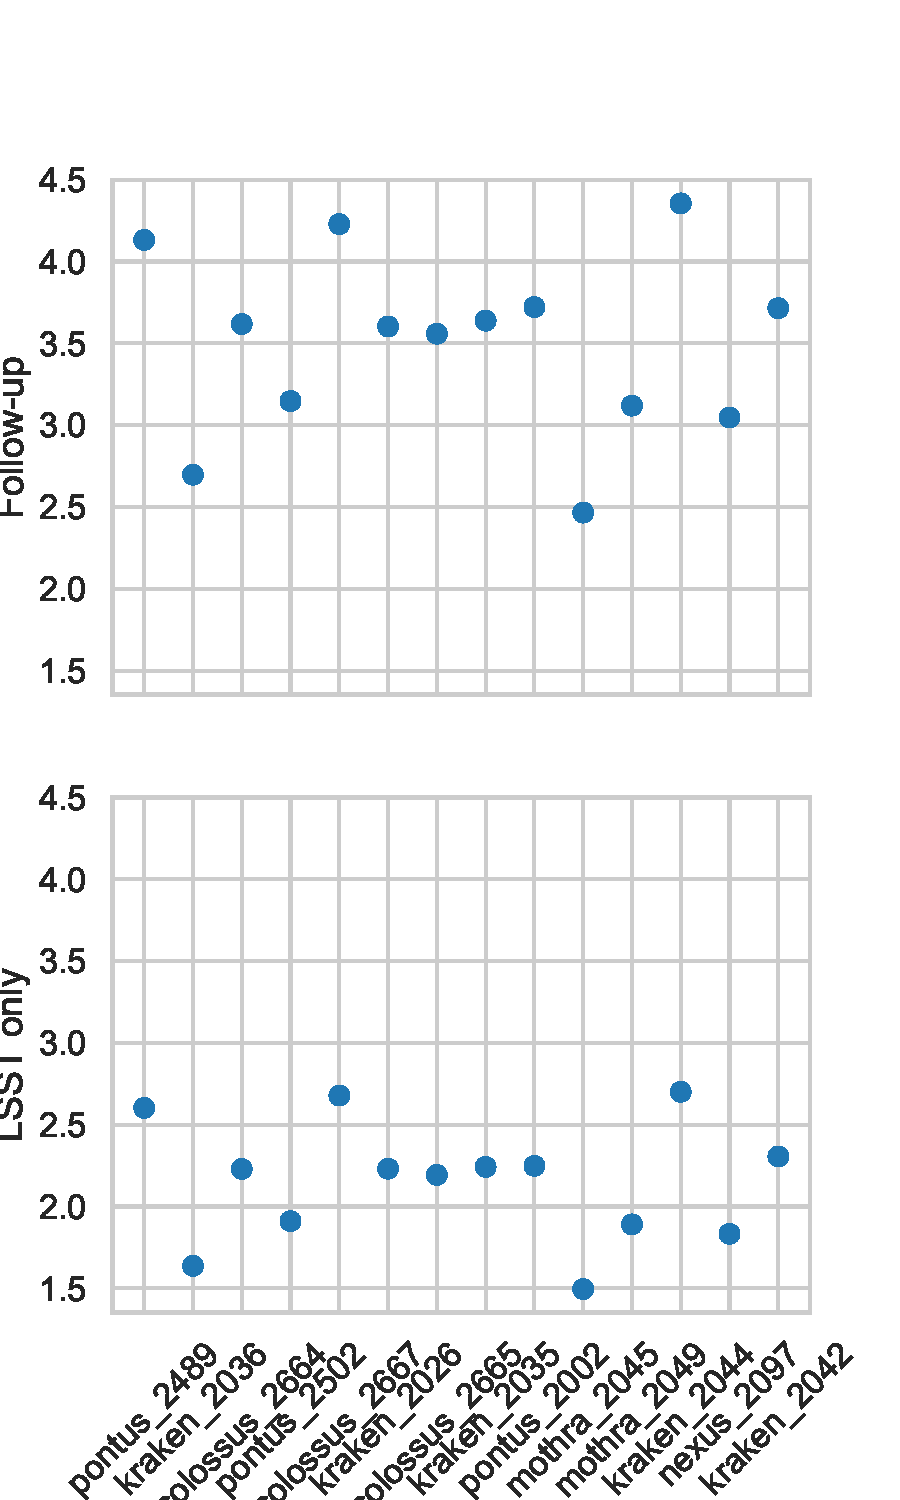
\includegraphics[width=0.4\textwidth]{peculiar_velocity/metrics.pdf}
        \caption{Fig.~Metrics for the strategies provided both in the case where follow-up with some other photometric telescope will characterize the light curves perfectly, and where only LSST photometry will be used}
    \label{fig:cadence_metrics}
    \end{center}
\end{figure}
%Our prescription reproduces the observed volumentric abundances of SNIa as observed in un-targetted rolling searches of SNIa in previous surveys. It should be noted that no extra-galactic catalog is large enough to cover the LSST sky area. Hence, we use scaling relations to go from a list of all of the SNIa realized in our presciption over the catalog light cone volume to the detected number of pairs in the LSST sky using different observing strategies. We describe the current state of these scaling relations and our approximations for this estimate. 

%Within the area of the galaxy catalog, we can count the number of SNIa pairs exploding throughout the survey separated a particular distance. We call this number $N_{pair}^{tV}$. Due to the survey strategy, we assume that of the N SNIa exploding through the survey period within a certain volume, we will only see $N_{det} = \epsilon N$ of them. Clearly, $\epsilon$ might be a function of SNIa properties, but we simply assume a flat efficiency of detection here. To count the number of pairs, we iterate over the detected SN and for each of them construct a spherical shell of radius $r Mpc$ and thickness $dr$. All SNIa that lie on this shell form a pair with the SN we are iterating over. Thus, the total number of pairs in a large enough volume where edge effects may be neglected is $2\times \pi r^2 dr \rho_{det} N_{det},$ where $N_{det}$ is the number of detected SNIa, $\rho_{det} = \epsilon N / V$ is the number density of SNIa over the survey period in this volume $V$

%First, we place SNIa in galaxies in a simulated extragalactic catalog of galaxies with different galaxy properties. The presecription we use to do this is simple, and can be varied later. However, the important factors to note are 
%\begin{enumerate}
%    \item these SNIa are meant to be all of the SNIa exploding during the survey and in the right range of redshift, but not all of them will be detected by LSST.
%    \item As the extra galactic catalog is only over a small area of the sky rather than the areas scanned by the Observing Strategies, we need to scale the numbers to find the appropriate $N(r,a).$
%\end{enumerate}

%If we assume that a fraction $\epsilon$ of the SN will be detected, since the number of pairs scales like $\mathcal{O}(N^2),$ the number of detected pairs in the fiducial area covered by the extra-galactic catalog scales as $\sim f^2.$ The efficiency $f$ can be estimated from the SNANA simulations by comparing the number of SNIa detected according to the simulations and the numbers simulated. Obviously this simple prescription misses some parameter dependence of the efficiency which we can return to for a more detailed calculation. Since the area scanned by the observing strategies are much larger than the separation in comoving distances at which we are considering pairs of SNIa, the increase in the number of pairs does not scale $\sim N^2 \sim \rm{Area}^2.$ Instead, if we can assume that the fiducial area is large enough that the edge effects are small for the largest separatation considered, and the shape of the larger area scanned by the observing strategy is not too irregular, we expect the number of pairs to scale $\sim \rm{Area}.$ Combining these considerations, we estimate that the number of pairs of detected SNIa at comoving distances of $r \rm{Mpc}$ at a cosmological redshift $z_{\rm{cosmo}}$ is given by 
%\begin{eqnarray}
%N = f^2 \frac{\rm{Cadence~Area}}{\rm{fiducial~area~of~extragalactic~Catalog}} N_{pairs}\\
%f  = \frac{\rm{Number~of~detected~SNIa~in~SNANA}}{\rm{Numbe~of~simulated~SNIa~in~SNANA}}
%\end{eqnarray}
